
%(BEGIN_QUESTION)
% Copyright 2011, Tony R. Kuphaldt, released under the Creative Commons Attribution License (v 1.0)
% This means you may do almost anything with this work of mine, so long as you give me proper credit

Your task is to sketch a workable PLC program to control the starting and stopping of a liquid-cooled grinding machine, given the following I/O connections and device statuses:

\begin{itemize}
\item{} {\bf Input card channels} 
\item{} {\tt Channel 1} = Start pushbutton (momentary NO) -- {\it pushing this button closes the switch to energize the PLC input}
\item{} {\tt Channel 2} = Stop pushbutton (momentary NC) -- {\it pushing this button opens the switch to de-energize the PLC input}
\item{} {\tt Channel 3} = Coolant flow switch (NO) -- {\it adequate coolant flow closes the switch to energize the PLC input}
\end{itemize}

\begin{itemize}
\item{} {\bf Output card channels} 
\item{} {\tt Channel 1} = Motor contactor -- {\it energizing this PLC output starts the grinding machine's motor, which also turns the coolant pump to spray liquid coolant on the grinding zone}
\end{itemize}

\vskip 10pt

Upon momentarily pushing the ``Start'' button, the grinding machine starts immediately, but will automatically shut down if low coolant flow is detected for more than 3 seconds continuously.  Pressing the ``Stop'' button shuts the grinding machine down regardless of coolant flow status.

$$\includegraphics[width=15.5cm]{i03552x01.eps}$$

Since you will not have access to PLC programming software during the exam, your address labeling and instruction syntax does not have to be 100\% perfect.  If you can't remember how the exact address is written for channel 3 on card 2 of an Allen-Bradley PLC, for example, or the displayed order of the parameters inside of a Siemens timer instruction, it's no big deal.  All that matters is that your program is clear and unambiguous.  Tagnames (e.g. ``{\tt Start\_switch}'') are recommended in lieu of model-specific address labels such as {\tt I0.6}.

\underbar{file i03552}
%(END_QUESTION)





%(BEGIN_ANSWER)

{\it Half-credit if any details (e.g. address labels, either hardware-oriented or tagname-oriented) are missing from the sketched program, assuming the basic structure of the program is sound.  No credit should be given for any program failing to properly implement \underbar{all} stated objectives.  If any stated objective will only be implemented inconsistently (rather than reliably, every time), award half-credit.  Deduct 1 point if any gratuitous output bits are used instead of ``internal'' bits.}

\vskip 10pt

Here is one sample program, for Allen-Bradley MicroLogix PLCs:

$$\includegraphics[width=15.5cm]{i03552x02.eps}$$

%(END_ANSWER)





%(BEGIN_NOTES)

{\bf This question is intended for exams only and not worksheets!}.

%(END_NOTES)

